%%%%%%%%%%%%%%%%%%%%%%%%%%%%%%%%%%%%%%%%%%%%%%%%%%%%%%%%%%%%%%%%%%%%%%%%%%%%%%%%
% EINSTELLUNGEN
%%%%%%%%%%%%%%%%%%%%%%%%%%%%%%%%%%%%%%%%%%%%%%%%%%%%%%%%%%%%%%%%%%%%%%%%%%%%%%%%

% Seitenränder:
\renewcommand{\SeitenrandOben}{33.5mm}
\renewcommand{\SeitenrandRechts}{20mm}
\renewcommand{\SeitenrandLinks}{20mm}
\renewcommand{\SeitenrandUnten}{10mm}

%\newcommand{\UniversitaetLogoBreite}{19mm}
%\newcommand{\UniversitaetLogoHoehe}{1cm}
%
%\newcommand{\StatikLogoBreite}{2.37cm}
%\newcommand{\StatikLogoHoehe}{0.95cm}

%\usepackage[a4paper,
%    top=\SeitenrandOben,
%    bottom=\SeitenrandUnten,
%    inner=\SeitenrandLinks,
%    outer=\SeitenrandRechts,
%    foot=0cm,
%    head=0cm
%]{geometry}

\newgeometry{
    top=\SeitenrandOben,
    bottom=\SeitenrandUnten,
    inner=\SeitenrandLinks,
    outer=\SeitenrandRechts,
    foot=0cm,
    head=0cm
}

\textblockorigin{\SeitenrandLinks}{\SeitenrandOben} % Ursprung für Positionierung

\setlength{\parindent}{0pt}
%\setlength{\baselineskip}{32pt}
\setlength{\parskip}{\baselineskip}
\TabPositions{4cm}
\pagestyle{empty}


%%%%%%%%%%%%%%%%%%%%%%%%%%%%%%%%%%%%%%%%%%%%%%%%%%%%%%%%%%%%%%%%%%%%%%%%%%%%%%%%
% DOKUMENT
%%%%%%%%%%%%%%%%%%%%%%%%%%%%%%%%%%%%%%%%%%%%%%%%%%%%%%%%%%%%%%%%%%%%%%%%%%%%%%%%

%\begin{document}
\definecolor{TUMblue}{RGB}{0,101,189}


%\begin{textblock*}{\UniversitaetLogoBreite}[1,0](\textwidth-1mm, 2cm-\SeitenrandOben)%
%    \raggedleft
\includegraphics{./Ressourcen/Universitaet_Logo_RGB.pdf}%
%\end{textblock*}

%\begin{textblock*}{\textwidth}[1,0](\textwidth-1mm, 2cm-\SeitenrandOben)%
%    \raisebox{-.5\height}{
\includegraphics[width=1.9cm]{./Ressourcen/Universitaet_Logo_RGB.pdf}}%
%    \hfill
%    \raisebox{-.5\height}{\includegraphics[width=2.37cm]{./Ressourcen/Statik.pdf}}%
%\end{textblock*}
%
%\vspace*{1mm}
%{\fontsize{50pt}{70pt}\selectfont\textbf{\Titel}}

%{\fontsize{50pt}{48pt}\selectfont\textbf{\Titel}\par}

\begin{textblock*}{1.0\textwidth}[0,0](0cm, 0cm)%
{\fontsize{50pt}{40pt}\selectfont\textbf{Advanced Shell \\ Finite Elements}\par}
{\fontsize{36pt}{30pt}\selectfont\textbf
	{\textcolor{gray75}{Formulation, \\ Implementation \& \\ Structural Modelling}}\par
}

%	{\textcolor{gray75}{\Untertitel}}\par


{\fontsize{24pt}{26pt}\selectfont\textbf{\textcolor{TUMblue}{Master's Thesis by Peter Wilson}}}
\end{textblock*}

\vspace*{102.2mm}
%\vspace*{82.2mm}

\begin{figure}[H]
	\centering
	\def\svgwidth{\columnwidth}
	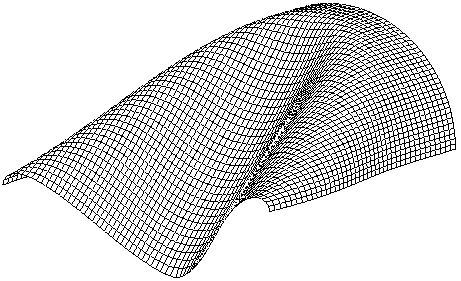
\includegraphics[width=\textwidth]{./Ressourcen/titleimage.pdf}
\end{figure}


\AddToShipoutPictureBG*{%
	\AtTextLowerLeft{\makebox[\textwidth][r]
		{%
			
\includegraphics[width=1.9cm]{./Ressourcen/Universitaet_Logo_RGB.pdf}
			\hspace{\fill}
			\includegraphics[width=2.37cm]{./Ressourcen/Statik.pdf}
		}
		}
		}

%\begin{textblock*}{\textwidth}[1,0](\textwidth-1mm, 2cm-\SeitenrandOben)%
%	\raisebox{-.5\height}{
\includegraphics[width=1.9cm]{./Ressourcen/Universitaet_Logo_RGB.pdf}}%
%	\hfill
%	\raisebox{-.5\height}{\includegraphics[width=2.37cm]{./Ressourcen/Statik.pdf}}%
%\end{textblock*}
%
%\includegraphics[width=4cm]{image1.eps}
%\hspace{\fill}
%\includegraphics[width=4cm]{image2.eps}

%\newpage

%\vspace*{-15.8mm}
%\fontsize{19pt}{21pt}\selectfont
%\ErklaerungUeberschrift
%
%\vspace{25.3mm}
%Erklärung
%
%\normalsize\selectfont
%\vspace{13.2mm}
%Ich versichere hiermit, dass ich die von mir eingereichte Abschlussarbeit selbstständig verfasst und keine anderen als die angegebenen Quellen und Hilfsmittel benutzt habe.
%
%\vspace{18.1mm}
%\rule[-3.7mm]{\linewidth}{0.5pt}
%\Ort{}, \Datum{}, Unterschrift

%\end{document}

\renewcommand{\SeitenrandOben}{25.8mm}
\renewcommand{\SeitenrandRechts}{21mm}
\renewcommand{\SeitenrandLinks}{40mm}
\renewcommand{\SeitenrandUnten}{24.8mm}

\restoregeometry
